
%*******************************************************************************
%***********************************    Background   *****************************
%*******************************************************************************
%!TEX root = 0.main.tex

\setcounter{page}{1}



%********************************** %First Section  **************************************
\section {Introduction and general background} 

\subsection{Introduction}

Neural Networks (NNs) are popular algorithms for regression and classification tasks. Taking as example an image classification problem, a neural network perform multiple combinations of linear and non-linear transformations of each image $I$ to assign it a label $C_I$ chosen in the set of all the possible labels $\mathcal C$. The first \textit{layer} of the neural network transforms the input image $I$ in a vector - called \textit{feature map} - $\mathbf f_1$ through a function $\phi_1$.  The output feature map of the first layer is used as input of the second layer that transforms it through a function $\phi_2$, and so on, until the original image $I$ is mapped into a label $C_I$ by the last, $n$-th layer of the neural network:
$$C_I = \phi_n \circ \phi_{n-1}\circ ... \phi_2\circ\phi_1 (I)$$
 With a large \textit{training set} of pre labeled images at its disposal, a NN is capable of learning the optimal transformations $\phi_i$ that let it map each input image to its correct label. Since the functions $\phi_i$ have many degrees of freedom - even millions - a neural network is able to learn very complex transformations. In the work of Cs\'aji \cite{NN}, NNs have been proved to be universal function approximators, meaning that with a sufficient number of parameters NNs are able to approximate any continuous function on a compact domain. This makes NNs the optimal tool for complex tasks such as image classification, image segmentation, speech recognition and natural language processing.
 
Convolutional Neural Networks (CNNs) are a subset of NNs whose layer structure has been specifically designed for image recognition and segmentation. For this purpose, they don't have all the degrees of freedom of a \textit{fully connected} neural network: each layer is constrained to learn only those transformations of the input that are \textit{equivariant} to translations of the input. This means that a translation of the input image will not result in a change of class. The layers $\phi_i$ of a CNN are \textit{convolutions} with some kernels $k_i$, that were learned during the training phase. Thanks to their design, training of CNNs is faster - thanks to the smaller number of parameters to be learned compared to a fully connected NN -, easier - since there's no need of artificially \textit{augmenting} the dataset with translated copies of the same image -, and leads to very accurate results \cite{SCNN}, \cite{Esteves}.

Spherical convolutional neural networks (SCNNs) are CNNs that have been designed to deal with spherical data, whose layer design makes them equivariant to \textit{rotations} of the input.  Examples of tasks where data is naturally represented on a sphere are (i) climate science, where data is sampled on the surface of the Earth, (ii) cosmology, where observations are naturally projected on a sphere centered around the observer (see Figure \ref{fig:cosmicradiation}), and (iii) virtual reality, where the images are represented on a sphere centered around the player. Being able to come up with rotation equivariant architectures brings with it all the advantages that traditional CNNs have brought for traditional (euclidean) image classification tasks: training is faster, easier and results are very accurate. Each layer of a SCNN performs a \textit{spherical convolution} of the input feature map with a kernel $k_i$ learned during the training phase. One of the main issues with traditional SCNNs is the computational complexity of computing at each layer the Spherical Harmonic Transform (SHT, equation \ref{eq:SHT}) of the data to perform the convolution. To overcome this issue, Perraudin et al. \cite{DeepSphere} proposed a Graph Convolutional Neural Network (GCNN) that is almost equivariant to rotations, replacing the SHT with a more efficient Graph Convolution.
\begin{figure}
	\centering
	\caption{\label{fig:cosmicradiation} Cosmic microwave background map, the oldest electromagnetic radiation in the universe. Source: Wikipedia}
	\includegraphics[width=0.4\textwidth]{figs/literaturereview/WMAP.png}
\end{figure}

This work is organized as follows: in Chapter 1 we start by presenting fundamental concepts of spectral theory on the sphere and we present classical ways of building rotation equivariant neural networks through the use of the classical SHT.  We present then some basics of Graph Spectral Theory that lay the foundations of Graph Convolutional Neural Networks.  In Chapter 2 we present the general framework of how to discretize the Laplace-Beltrami operator on a general manifold, concluding with the special case of the Heat Kernel Graph Laplacian (HKGL) approximation, together with some convergence results. We continue in Chapter 3 by introducing DeepSphere \cite{DeepSphere}, a Graph Spherical Convolutional Neural Networks that uses a graph Laplacian matrix $\mathbf L$ similar to the HKGL to perform graph convolutions that are almost equivariant to rotations. We study the spectral properties and the equivariance error of DeepSphere and we show a way to build a graph $G'$ such that the corresponding graph Laplacian matrix $\mathbf L'$ shows better spectral and equivariance properties. We conclude this chapter by presenting some experimental results obtained by Gusset et al. \cite{Gusset} that tested such architectures on the SHREC17 dataset \cite{SHREC17} showing that the new graph $G'$ performs better in real applications too. In Chapter 4 we show better graph constructions than the HKGL on non uniform sampling measures. To conclude, we show a different approach to perform rotation invariant convolutions that uses the Finite Element Method (FEM) approximation of the Laplace-Beltrami operator on the the sphere. Chapter 5 concludes this work by comparing the FEM and the graph approach, discussing the general problem of how to incorporate geometrical informations about the sphere in the graph.

\subsection{Fourier Transforms and Convolutions on the 2-Sphere}\label{sec:Fourier on the Sphere}
The goal of this section is to present to the reader some fundamental results of spectral theory on the sphere that we will need in this work. We present a brief review of Banach and Hilbert spaces, spherical harmonics, Fourier transform and convolution on $\mathbb S^2$. We refer to Sections 2 and 3 of the work of Driscoll and Healy \cite{Driscoll:1994:CFT:184069.184073} for a more detailed and effective review of spectral theory on the Sphere.

\paragraph{Banach and Hilbert spaces}
A \textit{norm} $\norm\cdot:\ X\to\mathbb R$ on a vector space $X$ is a subadditive, positive definite function such that $\norm{x+y}\leq\norm x +\norm y,\ \forall x,y\in X$ (triangle inequality). A \textit{Cauchy sequence} $(x_n)\subset X$ is a sequence such that $\forall \epsilon>0\  \exists M>0: $ $\forall i,j>M$ $ \norm{x_i-x_j}<\epsilon$. A \textit{Banach space} $(X, \norm{\cdot})$ is a normed vector space on the scalar field $F$ that is \textit{complete}, meaning that $X$ is "big enough" such that for every Cauchy sequence $(x_n)\subset X$ there exist a $x\in X$ such that $x$ is the limit of $(x_n)$ in $X$ i.e. $\norm{x_n-x}\rightarrow 0$. A \textit{basis} of $(X, \norm\cdot)$ is a minimal set of linearly independent vectors $\mathcal B \subset X$ such that every element of $X$ can be written as linear combination of the elements of $\mathcal B$. A scalar product is a function $\langle\cdot,\cdot\rangle: X\times X \rightarrow \mathbb F$ that is linear in the first argument, positive definite and conjugate symmetric. Through a scalar product we can define the notion of angle $\theta$ between two elements $x, y \in X$ through the following formula: 
$$
\cos \theta = \frac{\langle x, y\rangle}{\norm x \norm y}
$$ 
In particular we can define the notion of orthogonality: two elements  $x, y \in X$ are orthogonal if and only if $\langle x, y\rangle=0$. We are interested in those particular Banach spaces where we can define a notion of orthogonality between vectors. A Banach space $(X, \norm \cdot )$ is a \textit{Hilbert space} when the norm $ \norm \cdot $ can be induced by a \textit{scalar product}: $\norm \cdot = \sqrt{\langle\cdot,\cdot\rangle}$. We can now define an \textit{orthonormal} basis of $X$: a basis $\mathcal B \subset X$ such that $\forall x, y \in \mathcal B, \norm x = \norm y = 1 \text{and } \langle x, y\rangle = 0$. Given an orthonormal basis $\mathcal B = \{b_i\}_{i\in I}$ we can write each vector in its \textit{Fourier series} 
\begin{equation}\label{eq:abstract fourier}
x = \sum_{i\in I} \langle x, b_i\rangle b_i
\end{equation}
If the set $I$ is countable the Hilbert space $(X, \norm\cdot)$ is called \textit{separable}. Having a countable orthonormal basis, and thus the possibility of representing each vector through its Fourier series enormously simplifies many problems.
\paragraph{Spherical Harmonics}
 Given the usual parametrization $x = x(\theta, \phi), \theta\in[0,\pi], \phi\in[0,2\pi]$ of the sphere
\begin{align*}
\mathbb{S}^{2}&=\left\{\omega=\left(\omega_{1}, \omega_{2}, \omega_{3}\right) \in \mathbb{R}^{3} :\|x\|_{\mathbb{R}^{3}}=\left(\omega_{1}^{2}+\omega_{2}^{2}+\omega_{3}^{2}\right)^{1 / 2}=1\right\}\\
\omega_{1}&=\cos (\phi) \sin (\theta), \quad \omega_{2}=\sin (\phi) \sin (\theta), \quad \omega_{3}=\cos (\theta)
\end{align*}
the Hilbert space $L^2(\mathbb S^2)$ is defined as the space of square-integrable functions endowed with the scalar product $\langle f,g\rangle=\int_{\mathbb S^2}f(\omega)\overline g(\omega)d\omega$ where the measure $d\omega$ is the rotation-invariant measure such that
\begin{align}
\int_{\omega \in \mathbb S^{2}} f(\omega) d \omega&=\int_{\phi=0}^{2 \pi} \int_{\theta=0}^{\pi} f(\omega(\theta, \phi)) \sin \theta d \theta d \phi\\
\int_{\omega \in \mathbb S^{2}} f(g \omega) d \omega&=\int_{\omega \in \mathbb S^{2}} f(\omega) d \omega, \quad g \in S O(3)
\end{align}

For each rotation $g\in SO(3)$ we define a corresponding rotation operator $\Lambda(g)$ by
\begin{equation}\label{eq:rotation operator}
	\Lambda(g) f(\omega)=f\left(g^{-1} \omega\right)
\end{equation}
A space is invariant under the rotations $g$ in $SO(3)$ if all operators $\Lambda(g)$ take each function of the space back into the space. As very well written by Driscoll et al \cite{Driscoll:1994:CFT:184069.184073}:

\vspace{0.2cm}
\textit{Fourier analysis on the sphere amounts to the decomposition of the space of square integrable functions on \(\mathbb S^{2}\) in minimal subspaces $V_\ell$ invariant under all of the rotations in \(S O(3),\) thus simplifying the analysis of rotation-invariant operators.}
\vspace{0.2cm}

It's a well known fact \cite{Driscoll:1994:CFT:184069.184073} that the $\ell$-th invariant subspace $V_\ell\subset L^2(\mathbb S^2)$ is made of polynomials of $\mathbb R^3$ of degree $\ell$ restricted to $\mathbb S^2$, and has dimension $2\ell+1$. Its elements are called \textit{spherical harmonics} of degree $\ell$. These subspaces are orthogonal between them, and correspond to the eigenspaces of the Laplace-Beltrami operator $\Delta_{\mathbb S^2}$. For a thorough introduction to how to define the Laplace-Beltrami operator on a manifold and its properties, see \cite{rosenberg_1997}. The set of all the orthonormal basis $Y_\ell^m,\ -\ell\leq m\leq\ell$ of each subspace $V_\ell$ gives an orthonormal basis of $L^2(\mathbb S^2)$. The analytical expression of the spherical harmonic $Y_\ell^m(\theta, \phi)$ is actually known \cite{Driscoll:1994:CFT:184069.184073}:
\begin{equation}\label{eq:spherical harmonics}
	Y_\ell^m(\theta, \phi) = (-1)^{m} \sqrt{\frac{(2 \ell+1)(\ell-m) !}{4 \pi(\ell+m) !}} P_{\ell}^{m}(\cos \theta) e^{i m \phi}
\end{equation}
where $P_{\ell}^{m}$ are the \textit{Legendre functions} as defined in \cite{Driscoll:1994:CFT:184069.184073}. 
\vspace{0.5cm}
\begin{remark}
	Saying that the space $V_\ell$ is invariant under rotations $SO(3)$ means that under any rotation $g\in SO(3)$, any spherical harmonic $Y_\ell^m\in V_\ell$ is transformed into a linear combination of the others spherical harmonics of the same degree $\ell$:
	$$
	\Lambda(g) Y_{\ell}^{m}(\omega)=\sum_{|k| \leq \ell} Y_{\ell}^{k}(\omega) \alpha_{k, m}^{(\ell)}(g).
	$$
\end{remark}
\vspace{0.5cm}

\paragraph{Fourier transform}
We can now expand each function $f\in L^2(\mathbb S^2)$ in the orthonormal coordinate system given by the spherical harmonics 
\begin{align}\label{eq:inverse spherical fourier transform}
	f(\omega) &= \sum_{\ell\in\mathbb N}\sum_{|m|\leq \ell}\hat f(\ell,m) Y_\ell^m(\omega)\\
	\hat f(\ell,m) &=\int_{\omega\in\mathbb S^2}f(\omega)Y_\ell^m(\omega)d\omega \label{eq:SHT}
\end{align}
where the coefficients $\hat f(\ell,m)$ are the \textit{Fourier coefficients} of $f$. The computation of $\hat f(\ell, m)$ is called Spherical Harmonic Transform (SHT). Thanks to equation (\ref{eq:spherical harmonics}) we can decompose the computation of the SHT (\ref{eq:SHT}) in the two directions $(\theta, \phi)$. One reason for which the most popular samplings of the sphere have the pixels lie on isolatitude circles is that it is possible to use standard one-dimensional FFT algorithms to compute the longitudinal part of the transform \cite{HEALPix}.

\paragraph{Convolutions}
Convolution on the sphere is profoundly different than convolution on the Euclidean plane $\mathbb R^2$. Since translations are isomorphic to $\mathbb R^2$, the convolution $f*g(x)$ of two functions $f, g \in L^2(\mathbb R^2)$ is itself a function on the plane:
\begin{equation}\label{eq:plane convolution}
	 \int_{\mathbb R^2} f(y)g(x-y)dy = f*g(x):\quad \mathbb R^2 \to\mathbb R
\end{equation}
On the sphere things work differently: translations are replaced by rotations, but due to the fact that $SO(3)$ is not isomorphic to $\mathbb S^2$ if we define the convolution on $\mathbb S^2$ as follows:
\begin{equation} \label{eq:cohen convolution}
f* k(g) := \int_{\eta \in \mathbb S^2} \Lambda(g)k( \eta) f(\eta) d\eta=\int_{\eta \in \mathbb S^2} k(g^{-1} \eta) f(\eta) d\eta\\ 
\end{equation}
$f*k(g): SO(3)\to\mathbb R$ is not a function of the sphere anymore, but it is a function of the special rotation group $SO(3)$. In section \ref{sec:Chapter1:SCNN} we will explain how Cohen et al. \cite{SCNN} use in their work this definition of convolution on the sphere to construct a rotation equivariant NN. However, the definition of convolution that we will use in this work is the following, where the integral is performed not on the sphere but on the rotation group $SO(3)$:

\begin{equation}\label{eq:convolution}
 k * f(\omega)=\int_{g \in S O(3)} k(g \eta) f\left(g^{-1} \omega\right) d g 
\end{equation}

where $dg$ is the measure on $SO(3)$ that can be written in terms of the three Euler angles $(\theta, \phi, \psi)$ 
$$dg=\sin\theta d\theta d\phi d\psi$$
In this way $k * f(\omega)$ is still a function defined on $\mathbb S^2$. However, integrating on $SO(3)$ means integrating on the third Euler angle $\psi$, that in practice means using definition (\ref{eq:cohen convolution}) with the use of \textit{radial} kernels $k$ only.
Using the convolution defined in equation (\ref{eq:convolution}), the following theorem \cite{Driscoll:1994:CFT:184069.184073} generalizes on the sphere a well known property of convolutions and Fourier transforms: 
\vspace{0.5cm}
\begin{theorem}\label{theo:convolution}
	Given two functions $f, h$ in $L^2(\mathbb S^2)$, the Fourier transform of the convolution is a pointwise product of the transforms
$$
\hat{(f * h)}(\ell, m)=2 \pi \sqrt{\frac{4 \pi}{2 \ell+1}} \hat{f}(\ell, m) \hat{h}(\ell, 0).
$$
\end{theorem}
\vspace{0.5cm}

\subsection{Spherical Convolutional Neural Networks}\label{sec:Chapter1:SCNN}
Cohen et al. \cite{SCNN} proposed a NN where the first layer performs a convolution on the sphere of the input spherical signal with a spherical kernel as defined by equation (\ref{eq:cohen convolution}). The output feature map - a signal on $SO(3)$ - is processed by the deeper layers that perform other convolutions in $SO(3)$. All these convolutions are performed in the spectral domain as in theorem \ref{theo:convolution}, meaning that every signal has to be Fourier-transformed first, at each forward and backward step of the training phase of the NN. This approach, even with the use of Generalized FFT algorithms for $\mathbb S^2$ and $SO(3)$, remains both computationally expensive and memory expensive, due to the need of storing kernels defined on the much bigger space $SO(3)$. In section \ref{sec:Chapter2:Experimental validation} we report in table (\ref{tab:SHREC17_class}) the results of Gusset et al. \cite{Gusset}, that compared both the training and inference time of Cohen's SCNN, showing how slow this architecture is compared to other rotation equivariant NNs.
\subsection{Graph Spectral Theory} \label{sec:Chapter1: Spectral Graph Theory}
\paragraph{Graphs.}
For the purposes of this work, a \textit{weighted undirected graph} $G(V, E, \mathbf W)$ is defined by a vertex set $V$, an edge set $E$, where the edges are unordered pairs of vertices, and the matrix $\mathbf W$ whose entries $w_{ij}$ represent the weight of the edge $(v_i, v_j)$. $G$ is a \textit{simple} graph, if $w_{ij}$ assume only values in $\{0, 1\}$. Undirected graphs are common mathematical objects used to model simple, symmetric relationships between things. The edge $e_{ij} = (v_i, v_j) \in E$ is the mathematical object that translates the fact that the vertices $v_i, v_j$ are in a relationship, and the weight $w_{ij}$ measures how strong this relationship is. Common examples of graphs include friendship graphs, where people are the vertices and the edges represent friendship, or electric network graphs, where vertices represent electronic components and edges represent wires.
\paragraph{The graph Laplacian.}
If $\mathbf D$ is the diagonal matrix $\mathbf D_{ii} = \sum_j w_{ij}$, one can define \cite{Vandergheynst} the combinatorial graph Laplacian $\mathbf L$
\begin{equation}\label{eq:graph Laplacian}
		\mathbf L = \mathbf D-\mathbf W
\end{equation}
 and the symmetric normalized graph Laplacian $\mathbf L'$
\begin{equation}\label{eq:normalized graph Laplacian}
\mathbf L' =  \mathbf D^{-1/2}\mathbf L\mathbf D^{-1/2} = \mathbf I - \mathbf D^{-1/2}\mathbf W\mathbf D^{-1/2}
\end{equation}
In a simple friendship graph $G$, one can define a vector $\mathbf f$ such that each entry $ f_i$ is the age of the person associated with the vertex $v_i$, and could try to measure how much people tend to be friends with people of the same age. In other words, how smooth the signal $\mathbf f$ is on the graph $G$. A good measure for the smoothness of a signal on a graph is given by the \textit{Dirichlet energy} of the signal $\mathbf f$, i.e., the quadratic form associated with the normalized Laplace operator $\mathbf L'$:
\begin{equation}\label{eq:quadratic form}
	\mathbf f^T \mathbf L' \mathbf f = \sum_{\left(v_{j}, v_{k}\right) \in {E}} \frac{\boldsymbol{W}_{j k}}{\sqrt{d_{j} {d}_{k}}}\left({f}_{j}-{f}_{k}\right)^{2}
\end{equation}
The reason why the Dirichlet energy is a good measure of the smoothness of $\mathbf f$ is easier to understand in the case of a simple graph, where it reduces to the sum
\begin{equation}\label{eq:simple dirichlet energy}
	\mathbf f^T \mathbf L' \mathbf f = \sum_{\left(v_{j}, v_{k}\right) \in {E}} \left({f}_{j}-{f}_{k}\right)^{2}.
\end{equation}
 that will grow for each edge $(v_i, v_j)$ connecting people with very different age. Although the Dirichlet energy (\ref{eq:quadratic form}) works also for the combinatorial graph Laplacian $\mathbf L$, in practice it is preferred to use the symmetric normalized Laplacian when the degree distribution is wide. Another way of looking at equation (\ref{eq:simple dirichlet energy}) is as the following: the differences ${f}_j-{f}_k$ can be seen as the \textit{gradient} $\nabla \mathbf{f}$ that is a signal on the edges $(v_j, v_k)$ and equation (\ref{eq:simple dirichlet energy}) as the quadratic norm of such gradient $\norm {\nabla \mathbf{f}}^2$.
\paragraph{Graph Fourier transform}
Since the graph Laplacian is a symmetric matrix, we can write its eigen decomposition \cite{Strang}
$$
\mathbf L = \mathbf V\mathbf \Lambda\mathbf V^T
$$
 where $\mathbf V$ is the orthonormal basis of $\mathbb R^n$ of eigenvectors, and $\Lambda$ the real diagonal matrix of the eigenvalues $\Lambda = \text{diag}(\lambda_i\in \mathbb R)$. Similarly to the continuous domain, where the Fourier transform of a signal $f$ is defined as the projection of $f$ on the orthonormal eigenbasis of the Laplace-Beltrami operator $\Delta$, on a graph we can define a graph Fourier transform $\mathcal F_G: \mathbb R^n\to\mathbb R^n$ of a discrete signal $\mathbf f\in\mathbb R^n$ as the projection of $\mathbf f$ on the eigenvectors of the graph Laplacian $\mathbf L$:
\begin{equation}\label{eq:graph fourier}
\mathcal F_G(\mathbf f) := \mathbf V^T\mathbf f = \hat{\mathbf f}
\end{equation}
The inverse graph Fourier transform $\mathcal F^{-1}_G$ is thus 
\begin{equation}\label{eq:graph fourier inverse}
\mathcal F^{-1}_G(\hat{\mathbf f}) := \mathbf V \hat{\mathbf f} = \mathbf V\mathbf V^T\mathbf f = {\mathbf f}
\end{equation}
In the continuous case, the eigenvalues of the Laplace-Beltrami operator are associated with a notion of \textit{frequency} of the corresponding eigenfunction. In a graph we have a similar notion: define the Rayleigh quotient of a vector $\mathbf v \in \mathbb R^n$ to be
\begin{equation}\label{eq:Rayleigh}
	\mathcal R(\mathbf v) = \frac{\mathbf v^T\mathbf L \mathbf v}{\mathbf v^T\mathbf v}
\end{equation}
The well known \cite{Strang} Courant-Fischer characterization of eigenvalues and eigenvectors of symmetric matrices (\ref{eq:courantfisher}) can be interpreted in light of what we wrote about the interpretation of the Dirichlet energy (\ref{eq:quadratic form}) $\mathbf v^T \mathbf L \mathbf v$ as a measure of the smoothness of $\mathbf v$. The eigenvalue $\lambda_i$ is the measure of smoothness of the eigenvector $\mathbf v_i$, that is the smoothest vector perpendicular to the lower-degree eigenvectors $\mathbf v_1, ... \mathbf v_{i-1}$.
\begin{equation}\label{eq:courantfisher}
	\begin{aligned} 
	&\lambda_1 = \min_{\mathbf v\neq 0} \mathcal R(v)\\
	&\mathbf v_1 = \text{argmin}_{\norm {\mathbf v} = 1, \mathbf v\neq 0} \mathcal R(v)\\
	&\begin{cases}
	\lambda_i = \min_{\norm {\mathbf v} = 1, \mathbf v\perp \mathbf v_1, ..., \mathbf v_{i-1}} \mathcal R(v)\\
	\mathbf v_i = \text{arg min}_{\norm {\mathbf v} = 1, \mathbf v\perp \mathbf v_1, ..., \mathbf v_{i-1}}  \mathcal R(v)
	\end{cases}
	\end{aligned}	
\end{equation}
\begin{remark}
	It is interesting to notice that the Dirichlet energy of a signal $\mathbf f$ on a graph $G$ could change drastically by changing the underlying topology of $G$. In figure \ref{fig:graph} we see two simple graphs $G=(V, E),\ G' =(V, E')$ with the same signal $\mathbf f$ represented as vertical red bars over the vertex set $V$. On $G$, the signal $\mathbf f$ varies smoothly across the graph since the edges $V$ connect only those vertices with similar values of $\mathbf f$. On $G'$, since we added edges between vertices with very different values of $\mathbf f$, we will have that the Dirichlet energy of $\mathbf f$ calculated on the graph $G'$ will be much higher than the one calculated on the graph $G$
\end{remark}
\begin{figure}
	\centering
	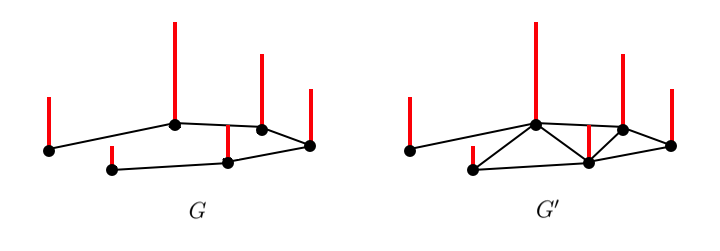
\includegraphics[width=0.8\textwidth]{figs/chapter1/graph.png}
	\caption{\label{fig:graph}Different graph topologies can drastically change the measure of smoothness of a signal $\mathbf f$, here represented as red vertical bars on the vertices.}
\end{figure}

\paragraph{Convolution and filtering on graphs}
 As the plane $\mathbb R^2$ is symmetric with respect to any translation and the sphere $\mathbb S^2$ is symmetric with respect to any rotation, the respective definitions of convolution (\ref{eq:plane convolution}), (\ref{eq:convolution}) are equivariant to the respective symmetry groups. Since there are no such global symmetries in a general graph $G$, definitions (\ref{eq:plane convolution}), (\ref{eq:convolution}) of convolutions on the spatial domain can not be extended naturally on graphs. However, both on $\mathbb R^2$ and on $\mathbb S^2$, the convolution of a signal $f$ with a kernel $k$ can be performed in the spectral domain by multiplying the transformed signal $\hat f$ times the transformed kernel $\hat k$: 
\begin{equation}\label{eq:convolution normal}
f*k = \mathcal F^{-1}(\hat f \cdot \hat k)
\end{equation}
In a similar way we can define a notion of convolution also in the graph spectral domain. We use the following definition \cite{Vandergheynst} of the convolution of a signal $\mathbf f$ times a kernel $\mathbf K$:
\begin{equation}\label{eq:graph convolution}
	\Omega_\mathbf K\mathbf f = \mathcal{F}^{-1}_G(\mathbf K \hat {\mathbf f})= \mathbf V\mathbf K  \mathbf V^T {\mathbf f}
\end{equation}
where $\mathbf K$ is a \textit{diagonal} \textit{matrix} $K_{ii} = k_i$. Graphs convolutions are different from the ones we are used to define in Euclidean domains (\ref{eq:plane convolution}), since the graph kernels $\mathbf K$ are diagonal matrices that can not be thought as the Fourier transform of a corresponding kernel defined in the spatial (vertex) domain. The diagonal elements $k_{i}$ can be thought as functions of the corresponding eigenvalues 
$$
k_{i}= k(\lambda_i)
$$
thus providing an intuitive frequency interpretation of the kernel $\mathbf K$. In this way the convolution can be seen as a \textit{filtering} operation: for example, a kernel $k(\lambda_i) = \exp (-\lambda_i)$ will be the kernel of a low-pass filter since it will cut the high frequencies.
